\documentclass[tikz,border=8pt]{standalone}
\usepackage[T1]{fontenc}
\usepackage[utf8]{inputenc}
\usepackage{amsmath,amssymb}
\usetikzlibrary{arrows.meta,calc}

\begin{document}
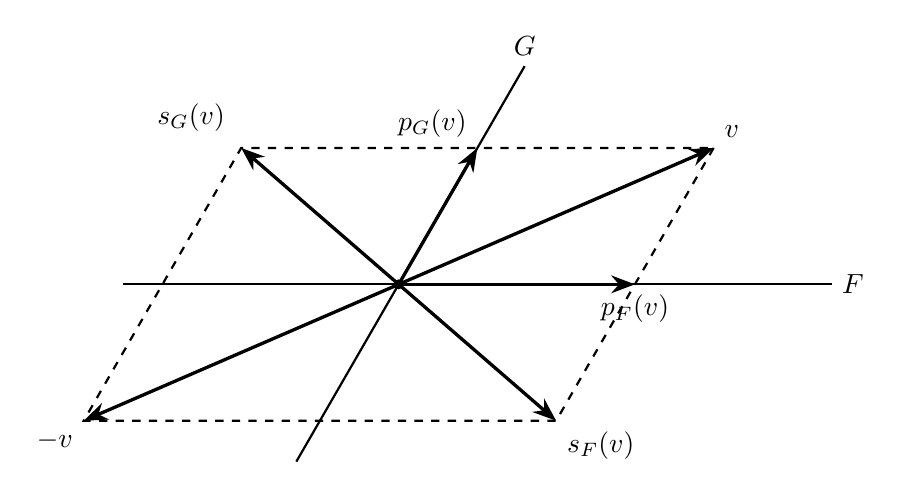
\begin{tikzpicture}[
  >={Stealth[length=3mm]},
  droite/.style={thick},
  vect/.style={very thick,->},
  fl/.style={->,thin},
]
  % Coordonnees
  \coordinate (O)  at (0,0);
  \coordinate (vF) at (3,0);    % composante suivant F
  \coordinate (vG) at (60:2);   % composante suivant G
  \coordinate (v)  at ($(vF)+(vG)$);
  \coordinate (sF) at ($(vF)-(vG)$); % symetrie / F // G : v_F - v_G
  \coordinate (sG) at ($(vG)-(vF)$); % symetrie / G // F : v_G - v_F
  \coordinate (mv) at ($(O)!-1!(v)$); % -v = -(v_F+v_G)

  % Sous-espaces F et G (droites vectorielles)
  \draw[droite] (-3.5,0) -- (5.5,0) node[right] {$F$};
  \draw[droite] (60:-2.6) -- (60:3.2) node[above] {$G$};

  % Parallelogramme (traits pointilles) : v, s_F(v), -v, s_G(v)
  \draw[dashed,thick] (v) -- (sF) -- (mv) -- (sG) -- cycle;

  % Vecteurs
  \draw[vect] (O) -- (v)  node[above right] {$v$};
  \draw[vect] (O) -- (vF) node[below] {$p_F(v)$};
  \draw[vect] (O) -- (vG) node[above left] {$p_G(v)$};
  \draw[vect] (O) -- (sF) node[below right] {$s_F(v)$};
  \draw[vect] (O) -- (sG) node[above left=2pt] {$s_G(v)$};
  \draw[vect] (O) -- (mv) node[below left] {$-v$};

  % Origine
  \fill (O) circle (1.8pt);
\end{tikzpicture}
\end{document}
